% 第8章第3节：函数类的紧性与覆盖数（Arzelà--Ascoli判据、覆盖数与度量熵、覆盖数的估计）。

\section{函数类的紧性与覆盖数}
\label{sec:apx-function-classes}

前两节始终固定一个目标：先给定$f$，再为它挑选近似，近似的预算可以依赖$f$。现在改为预先给定一个函数类$\mathcal F$，要求一套有限的代表同时服务于类中所有成员。量词的次序随之改变：“对每个$f$，存在有限表示”与“存在一套有限代表，对每个$f$都有一个靠近它的代表”是两个不同的命题。后者成立与否，取决于所用的距离以及类中函数共同受到的幅度和正则性约束。

第~\ref{chap:linear-functionals-operators}章的弱紧性不能代替这里的判断。在无限维Hilbert空间中，标准正交序列$(e_n)$有界并弱收敛到零（第~\ref{sec:lfo-weak-subsequence}节），但$\|e_n-e_m\|=\sqrt2$（$n\ne m$），没有按范数收敛的子列，单位球也不能被有限个半径小于$\sqrt2/2$的球覆盖。弱拓扑下的紧性针对较弱的收敛方式；在一致距离或$L^2$距离下能否有限覆盖，需要另外判断。本节先刻画一致距离下的相对紧性，再计量覆盖所需代表的个数。

\subsection{一致有界与等度连续}
\label{sec:apx-arzela-ascoli}

\paragraph{有界不足以抽出一致收敛子列}

在有限维空间中，有界序列总有收敛子列。在$C([0,1])$中这一点不再成立。考虑$f_n(x)=x^n$，它们都满足$\|f_n\|_\infty=1$。逐点地看，$x\in[0,1)$时$x^n\to0$，而$f_n(1)=1$，逐点极限是在$x=1$处跳到$1$的不连续函数。若某个子列一致收敛，其极限连续（一致极限保持连续性，可参考\BookChapterRef{chap:limits-continuity}{卷一“极限与连续”章}），又必须等于逐点极限，这是矛盾。所以$(x^n)$没有一致收敛的子列。

图~\ref{fig:apx-xn-powers}显示了问题出在哪里：$n$越大，函数在$x=1$附近从接近$0$升到$1$所用的区间越窄。每个$x^n$各自连续，但它们的连续性尺度没有共同的下界。

\begin{figure}[!htb]
  \centering
  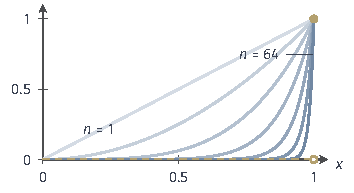
\includegraphics[width=60.0mm]{figures/02-abstract-mathematics/03-function-spaces/tikz/c6-xn-powers/figure.pdf}
  \caption{$[0,1]$上的$x^n$，$n=1,2,4,\ldots,64$（颜色由浅到深）。函数族一致有界，逐点极限在$[0,1)$上为$0$、在$x=1$处为$1$（黄色），不连续，因此没有一致收敛的子列；陡升区间随$n$变窄，族缺少共同的连续性尺度。}
  \label{fig:apx-xn-powers}
\end{figure}

\paragraph{等度连续}

缺少的条件是整个族共用一个连续性尺度。

\begin{definition}[一致有界与等度连续]
\label{def:apx-equicontinuous}
设$(X,d)$是度量空间，$\mathcal F$是$X$上的一族实值函数。若存在$M$使$|f(x)|\le M$对所有$f\in\mathcal F$、$x\in X$成立，称$\mathcal F$\term{一致有界}（uniformly bounded）。若对每个$\varepsilon>0$存在$\delta>0$，使
\[
  d(x,y)<\delta\ \Longrightarrow\ |f(x)-f(y)|<\varepsilon\qquad\text{对所有}f\in\mathcal F,
\]
称$\mathcal F$\term{等度连续}（equicontinuous）。
\end{definition}

与单个函数的一致连续相比，关键在于$\delta$只依赖$\varepsilon$，不依赖$f$。用连续模的语言，等度连续就是$\sup_{f\in\mathcal F}\omega_f(\delta)\to0$。最常见的例子是共用一个Lipschitz常数的族：若每个$f\in\mathcal F$都满足$|f(x)-f(y)|\le Ld(x,y)$，取$\delta=\varepsilon/L$即可。

反例来自没有共同尺度的族。$(x^n)$不等度连续：对任意$\delta\in(0,1)$，取$x=1$、$y=1-\delta/2$，则$|f_n(x)-f_n(y)|=1-(1-\delta/2)^n\to1$。图~\ref{fig:apx-equicontinuity}比较了两族函数在同一个宽$0.1$的窗口内的振幅：(a)中四个函数的Lipschitz常数都是$0.8\pi$，窗口内振幅都不超过$0.26$；(b)中$0.5+0.5\sin(2\pi nx)$的频率增长，$n=16$时在窗口内已扫过整个$[0,1]$。

\begin{figure}[!htb]
  \centering
  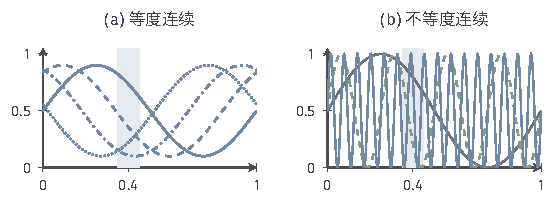
\includegraphics[width=94.2mm]{figures/02-abstract-mathematics/03-function-spaces/tikz/c6-equicontinuity/figure.pdf}
  \caption{共同连续性尺度的有无。蓝底为窗口$[0.35,0.45]$。(a)~$0.5+0.4\sin(2\pi x+a)$，$a=0,1,2,3$，共用Lipschitz常数$0.8\pi$，窗口内振幅都不超过$0.26$，族等度连续。(b)~$0.5+0.5\sin(2\pi nx)$，$n=1,4,16$，频率越高窗口内振幅越大，$n=16$时已达到$1$，族不等度连续。}
  \label{fig:apx-equicontinuity}
\end{figure}

\paragraph{Arzelà--Ascoli判据}

在紧度量空间上，一致有界与等度连续恰好刻画了一致距离下的相对紧性。回忆$C(X)$在一致范数下完备（第~\ref{sec:fs-uniform-norm}节）；子集称为\term{相对紧}（relatively compact），若它的闭包是紧集。

\begin{theorem}[Arzelà--Ascoli判据]
\label{thm:apx-arzela-ascoli}
设$(X,d)$是非空紧度量空间，$\mathcal F\subseteq C(X)$。则$\mathcal F$在一致范数下相对紧，当且仅当$\mathcal F$一致有界且等度连续。若$\mathcal F$还是闭集，则它是紧集。
\end{theorem}

证明的核心是一个有限化的机制：等度连续允许只在有限个位置上观察函数，一致有界允许把这些位置上的值量化为有限个等级，于是整个族只产生有限种“记录”。

\begin{proof}
充分性。设$|f|\le M$对所有$f\in\mathcal F$成立，并给定$\varepsilon>0$。由等度连续取$\delta>0$，使$d(x,y)<\delta$时$|f(x)-f(y)|<\varepsilon/4$对所有$f$成立。$X$紧，因而全有界，存在有限个点$x_1,\ldots,x_p$，使每个$x$都满足某个$d(x,x_i)<\delta$。再把$[-M,M]$分成有限个长度为$\varepsilon/4$的左闭右开小区间（最后一段含右端点），对每个$f$记下$f(x_1),\ldots,f(x_p)$各落在哪个小区间，称为$f$的记录。记录至多有$(\lceil8M/\varepsilon\rceil)^p$种，是有限个。

对每一种实际出现的记录，从$\mathcal F$中取一个具有该记录的成员作为代表。若$f$与代表$g$记录相同，则$|f(x_i)-g(x_i)|<\varepsilon/4$对每个$i$成立。对任意$x$取$x_i$使$d(x,x_i)<\delta$，
\[
  |f(x)-g(x)|\le|f(x)-f(x_i)|+|f(x_i)-g(x_i)|+|g(x_i)-g(x)|<\frac{3\varepsilon}4 .
\]
因此有限个代表构成$\mathcal F$的有限$\varepsilon$网，$\mathcal F$全有界。全有界集的闭包仍全有界（把每个球的半径放大一倍即可），而闭包是完备空间$C(X)$的闭子集，因而完备。由定理~\ref{thm:metric-compact-complete-tb}，闭包紧致。

必要性。设$\overline{\mathcal F}$紧，则$\mathcal F$全有界。取有限$\varepsilon/3$网$f_1,\ldots,f_N\in\mathcal F$。有界性：每个$f$都在某个$f_j$的$\varepsilon/3$邻域内，故$\|f\|_\infty\le\max_j\|f_j\|_\infty+\varepsilon/3$。等度连续：每个$f_j$在紧集上一致连续（定理~\ref{thm:metric-compact-uniform}），取$\delta$对这有限个函数同时适用，使$d(x,y)<\delta$时$|f_j(x)-f_j(y)|<\varepsilon/3$。对任意$f$选$f_j$使$\|f-f_j\|_\infty<\varepsilon/3$，则
\[
  |f(x)-f(y)|\le|f(x)-f_j(x)|+|f_j(x)-f_j(y)|+|f_j(y)-f(y)|<\varepsilon .
\]
最后，若$\mathcal F$闭，则$\mathcal F=\overline{\mathcal F}$紧。
\end{proof}

必要性的论证说明了有限网的作用：有限个函数总能共用一个$\delta$，再借助一致距离把这个$\delta$传给整个族。充分性中的位置网格和数值量化则是一个可以计数的构造，第~\ref{sec:apx-covering-estimates}节将用它给出Lipschitz类覆盖数的显式上界，图~\ref{fig:apx-lipschitz-quantization}画出了这个构造。

\paragraph{核范数有界球的一致紧性}

第~\ref{chap:rkhs}章的两个不等式恰好提供了Arzelà--Ascoli判据的两个条件。设$X$是紧度量空间，$K$是$X$上的连续半正定核，$B_R=\{f\in H_K:\|f\|_{H_K}\le R\}$。

\begin{theorem}[核范数球在连续函数空间中的紧性]
\label{thm:apx-rkhs-ball-compact}
在上述条件下，$B_R$是$C(X)$中按一致范数的紧集。
\end{theorem}

\begin{proof}
一致有界：由点值界（第~\ref{sec:rkhs-kernel-properties}节），$|f(x)|\le\|f\|_{H_K}\sqrt{K(x,x)}\le R\max_{X}\sqrt{K(x,x)}$，右端有限，因为连续函数在紧集上有最大值。

等度连续：由再生关系，
\[
  \begin{aligned}
  |f(x)-f(y)|&=|\langle f,K_x-K_y\rangle_{H_K}|\le R\,\|K_x-K_y\|_{H_K}\\
  &=R\sqrt{K(x,x)+K(y,y)-2K(x,y)} .
  \end{aligned}
\]
右端是$X\times X$上的连续函数，在对角线上为零。它在紧集$X\times X$上一致连续，所以存在$\delta$，使$d(x,y)<\delta$时右端小于$\varepsilon$，且$\delta$与$f\in B_R$无关。这里同时得到$B_R\subseteq C(X)$。

闭性：设$f_n\in B_R$且一致收敛到$g\in C(X)$。$(f_n)$在$H_K$中有界，由第~\ref{sec:lfo-weak-subsequence}节，存在子列弱收敛到某个$h\in H_K$；弱极限的范数不超过序列范数的下极限（第~\ref{sec:lfo-weak-norm}节），故$\|h\|_{H_K}\le R$。弱收敛蕴含$f_{n_k}(x)=\langle f_{n_k},K_x\rangle\to\langle h,K_x\rangle=h(x)$，而$f_{n_k}(x)\to g(x)$，所以$g=h\in B_R$。由定理~\ref{thm:apx-arzela-ascoli}，$B_R$紧。
\end{proof}

这个定理改变的是评价距离。$B_R$在一致距离下紧，并不意味着它在$H_K$自身的范数下紧：若$H_K$无限维，取其中的标准正交序列$(e_n)$，它们都在$B_1$中，彼此的核范数距离为$\sqrt2$，没有核范数收敛的子列。$[0,1]$上的高斯核就是这种情形：对互异中心$c_1,\ldots,c_M$，若$\sum_\ell a_\ell K_\sigma(\cdot,c_\ell)\equiv0$，乘以$e^{x^2/(2\sigma^2)}$后得到指数和$\sum_\ell a_\ell e^{-c_\ell^2/(2\sigma^2)}e^{c_\ell x/\sigma^2}\equiv0$，由引理~\ref{lem:apx-exponential-sum-zeros}全部$a_\ell=0$，所以$H_K$含有任意多个线性无关元素。

定理~\ref{thm:apx-rkhs-ball-compact}也补全了第~\ref{sec:apx-kernel-sections}节留下的论断：$B_R$在$C([0,1])$中闭且只含$H_K$的元素，$f_*\notin H_K$，所以$f_*$到$B_R$有正的一致距离。对任何固定的核范数预算$R$，有限核和都不能任意逼近$f_*$。

\subsection{覆盖数与度量熵}
\label{sec:apx-covering}

紧性回答“能否用有限个代表统一逼近”，没有回答“需要多少个”。本小节把代表的个数作为精度的函数记录下来。

\paragraph{覆盖数的定义与量词}

\begin{definition}[覆盖数与度量熵]
\label{def:apx-covering-number}
设$\mathcal F$是非空集合，$d$是$\mathcal F$上的距离或伪距离，$\varepsilon>0$。若有限集$V\subseteq\mathcal F$使每个$f\in\mathcal F$都有$v\in V$满足$d(f,v)\le\varepsilon$，称$V$为$\mathcal F$的一个$\varepsilon$覆盖。最小的覆盖规模
\[
  N(\varepsilon,\mathcal F,d)=\min\bigl\{|V|:V\text{是}\mathcal F\text{的}\varepsilon\text{覆盖}\bigr\}
\]
称为\term{覆盖数}（covering number），不存在有限覆盖时记为$+\infty$。其对数$\log N(\varepsilon,\mathcal F,d)$称为\term{度量熵}（metric entropy）。
\end{definition}

定义的量词是
\[
  \exists\ \text{有限}\ V\subseteq\mathcal F,\quad\forall f\in\mathcal F,\quad\exists v\in V:\ d(f,v)\le\varepsilon .
\]
代表集$V$必须在看到具体的$f$之前就固定下来，而且对类中每个成员都有效；只对大多数成员有效、或平均意义下有效，都不满足要求。每个$f$可以选择自己的近邻代表，但只能从$V$中选。

这里约定代表属于$\mathcal F$本身。若允许代表取自更大的空间，所得的外部覆盖数$N^{\mathrm{ext}}$可能更小，但两者只差精度的一个因子：
\[
  N^{\mathrm{ext}}(\varepsilon)\le N(\varepsilon)\le N^{\mathrm{ext}}(\varepsilon/2).
\]
第一个不等式显然。第二个：取一个外部$\varepsilon/2$覆盖，对每个与$\mathcal F$相交的球选一个类内成员替换球心，由三角不等式，原来落在该球中的成员到新代表的距离不超过$\varepsilon$。比较不同文献中的数值时，要先核对采用的是哪种约定。

\paragraph{覆盖数与全有界、紧性}

覆盖数把全有界的定义量化了。$\mathcal F$在$d$下全有界（定义~\ref{def:metric-totally-bounded}），当且仅当对每个$\varepsilon>0$都有$N(\varepsilon,\mathcal F,d)<\infty$：闭球$\{d(f,v)\le\varepsilon/2\}$含于开球$\{d(f,v)<\varepsilon\}$，开球又含于同半径的闭球，所以开球与闭球给出的有限性相同。若$\mathcal F$位于一个完备度量空间中，由定理~\ref{thm:metric-compact-complete-tb}，覆盖数处处有限等价于$\mathcal F$相对紧。结合定理~\ref{thm:apx-arzela-ascoli}，紧度量空间上一致有界且等度连续的函数族，在一致距离下对每个精度都有有限覆盖数。

伪距离允许$d(f,g)=0$而$f\ne g$。此时覆盖数只计及零距离等价类：彼此距离为零的成员共用同一个代表，因此应在第~\ref{sec:metric-pseudometric}节的商空间上理解覆盖数及其与紧性的关系。

\paragraph{三种距离的比较}

同一个函数类在不同距离下的覆盖数可以截然不同。设$X$上有概率测度$\mu$，又固定样本点$x_1,\ldots,x_n\in X$。三个常用的距离或伪距离为
\[
  \begin{aligned}
  d_\infty(f,g)&=\sup_{x\in X}|f(x)-g(x)|,\qquad
  d_{L^2(\mu)}(f,g)=\|f-g\|_{L^2(\mu)},\\
  d_n(f,g)&=\Bigl(\frac1n\sum_{i=1}^n\bigl(f(x_i)-g(x_i)\bigr)^2\Bigr)^{1/2}.
  \end{aligned}
\]
由于$\mu(X)=1$，后两者都不超过$d_\infty$。距离越弱，$\varepsilon$球越大，因此
\[
  N(\varepsilon,\mathcal F,d_{L^2(\mu)})\le N(\varepsilon,\mathcal F,d_\infty),\qquad
  N(\varepsilon,\mathcal F,d_n)\le N(\varepsilon,\mathcal F,d_\infty).
\]

经验距离$d_n$只看样本点，所以通常只是伪距离。图~\ref{fig:apx-empirical-distance}中$g(x)=0.3+0.4x$与$f(x)=g(x)+0.35\sin(5\pi x)$在六个样本点$0,0.2,\ldots,1$处取值相同，$d_n(f,g)=0$，但$d_\infty(f,g)=0.35$。

\begin{figure}[!htb]
  \centering
  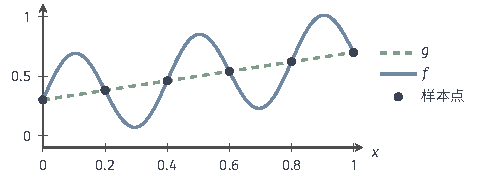
\includegraphics[width=81.2mm]{figures/02-abstract-mathematics/03-function-spaces/tikz/c6-empirical-distance/figure.pdf}
  \caption{经验距离只看样本点。$g(x)=0.3+0.4x$（虚线）与$f(x)=g(x)+0.35\sin(5\pi x)$（实线）在样本点$0,0.2,\ldots,1$（黑点）处相等，经验距离为$0$，一致距离却为$0.35$。}
  \label{fig:apx-empirical-distance}
\end{figure}

反方向的比较不成立，而且差距可以是有限与无穷之别。令$\mathcal F$为全体取值于$[0,1]$的连续函数。在$d_n$下，每个$f$由向量$(f(x_1),\ldots,f(x_n))\in[0,1]^n$决定距离；把每个坐标量化到$\lceil1/(2\varepsilon)\rceil$个等距点之一，所得网格点都是某个连续函数的样本值，于是$N(\varepsilon,\mathcal F,d_n)\le\lceil1/(2\varepsilon)\rceil^n<\infty$。在$d_\infty$下，取支撑互不相交的帽形函数列$(\phi_k)$，峰值为$1$，则$d_\infty(\phi_k,\phi_l)=1$（$k\ne l$），任何半径$1/3$的球至多含其中一个，所以$N(1/3,\mathcal F,d_\infty)=\infty$。样本上的记录有限，不能推出整个定义域上的有限覆盖；要从有限位置控制全域，需要等度连续这样的共同正则性，这正是定理~\ref{thm:apx-arzela-ascoli}的作用。

\subsection{覆盖数的估计与适用范围}
\label{sec:apx-covering-estimates}

本小节对几类具体的函数类估计覆盖数，观察它怎样依赖函数的幅度、参数维数、正则性和定义域。

\paragraph{常值族}

先看最简单的一维情形。设$X$非空，$M>0$，$\mathcal F_M=\{f_a\equiv a:a\in[0,M]\}$，距离取$d_\infty$。两个常值函数的距离就是$|a-a'|$，所以问题化为用半径$\varepsilon$的闭区间覆盖$[0,M]$。

下界由长度比较给出：每个代表$c$只覆盖长度为$2\varepsilon$的参数区间$[c-\varepsilon,c+\varepsilon]$，$N$个代表覆盖的总长度至多$2N\varepsilon$，必须不小于$M$。上界由均匀分点给出：令$N=\lceil M/(2\varepsilon)\rceil$，取$c_j=(2j-1)M/(2N)$，$j=1,\ldots,N$，相邻代表间距为$M/N\le2\varepsilon$，每个参数到最近代表的距离不超过$M/(2N)\le\varepsilon$。因此
\[
  N(\varepsilon,\mathcal F_M,d_\infty)=\Bigl\lceil\frac{M}{2\varepsilon}\Bigr\rceil,
\]
图~\ref{fig:apx-constant-cover}画出$M=1$、$\varepsilon=0.15$时的四个代表。

\begin{figure}[!htb]
  \centering
  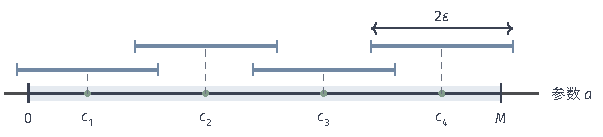
\includegraphics[width=102.2mm]{figures/02-abstract-mathematics/03-function-spaces/tikz/c6-constant-cover/figure.pdf}
  \caption{常值族$f_a\equiv a$（$a\in[0,1]$）在一致距离下的覆盖，精度$\varepsilon=0.15$。每个代表$c_j$（绿点）只覆盖长度$2\varepsilon$的参数区间（蓝色线段，上下错开以便辨认）；四个代表的总长度$1.2$不小于$1$，而三个只有$0.9$，所以覆盖数恰为$\lceil1/(2\varepsilon)\rceil=4$。}
  \label{fig:apx-constant-cover}
\end{figure}

这个例子已经显示了幅度的作用。参数个数固定为一个，把幅度$M$放大，覆盖数随$M$线性增长；一般地，对任意类$\mathcal F$和$B>0$，$N(\varepsilon,B\mathcal F,d_\infty)=N(\varepsilon/B,\mathcal F,d_\infty)$。度量熵$\log\lceil M/(2\varepsilon)\rceil$则只按$\log(1/\varepsilon)$增长。

\paragraph{有限维参数族}

再看两个参数的情形。设$\mathcal F=\{f_{a,b}(t)=a+bt:(a,b)\in[-1,1]^2\}$，$t\in[-1,1]$，距离取$d_\infty$。差$(a-a')+(b-b')t$是$t$的一次函数，绝对值的最大值在端点取得，等于$|a-a'|+|b-b'|$。因此一致距离恰好是系数平面上的$\ell^1$距离，$\varepsilon$球是菱形。

上界：把$[-1,1]$等分为$\lceil2/\varepsilon\rceil$段，取各段中点，每段长度不超过$\varepsilon$，所以每个坐标到最近中点的距离不超过$\varepsilon/2$。两个坐标方向的中点组成网格，每个系数点到最近网格点的$\ell^1$距离不超过$\varepsilon$，故$N(\varepsilon)\le\lceil2/\varepsilon\rceil^2$。下界：每个菱形面积为$2\varepsilon^2$，覆盖面积为$4$的正方形至少需要$4/(2\varepsilon^2)=2/\varepsilon^2$个。于是
\[
  \frac2{\varepsilon^2}\le N(\varepsilon,\mathcal F,d_\infty)\le\Bigl\lceil\frac2\varepsilon\Bigr\rceil^2,
\]
覆盖数按$\varepsilon^{-2}$增长，指数$2$正是参数个数。图~\ref{fig:apx-covering-centers}画出$\varepsilon=1/2$时的$16$个代表：(a)是系数平面上的菱形覆盖，(b)是对应的函数。

\begin{figure}[!htb]
  \centering
  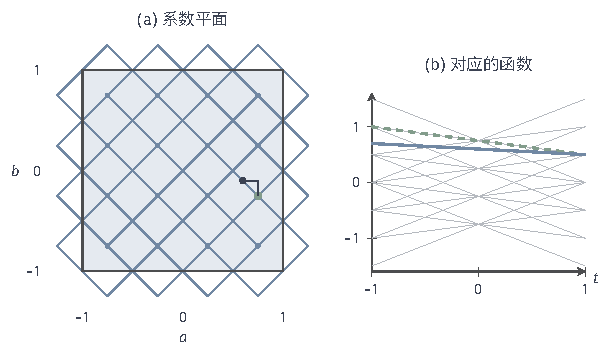
\includegraphics[width=103.2mm]{figures/02-abstract-mathematics/03-function-spaces/tikz/c6-covering-centers/figure.pdf}
  \caption{仿射函数类$a+bt$（$(a,b)\in[-1,1]^2$，$t\in[-1,1]$）的$\tfrac12$覆盖。(a)~一致距离等于系数的$\ell^1$距离，$16$个中心$\{\pm\frac14,\pm\frac34\}^2$的半径$\frac12$菱形覆盖整个正方形；黑点$(0.6,-0.1)$到最近中心$(\frac34,-\frac14)$（绿）的$\ell^1$距离为$0.3$。(b)~对应的函数：$16$条中心直线（细灰），成员$0.6-0.1t$（蓝）与其代表$0.75-0.25t$（绿虚线）的一致距离为$0.3$，在$t=-1$处取得。}
  \label{fig:apx-covering-centers}
\end{figure}

同样的论证适用于一般的有限维参数族。设$\mathcal F=\{\sum_{i=1}^p\theta_i\varphi_i:\|\bm\theta\|_\infty\le B\}$，$\varphi_i$有界，令$\Lambda=\sup_x\sum_i|\varphi_i(x)|$。则$d_\infty(f_{\bm\theta},f_{\bm\theta'})\le\Lambda\|\bm\theta-\bm\theta'\|_\infty$，把参数立方体$[-B,B]^p$在每个坐标上按精度$\varepsilon/\Lambda$分点，得到
\[
  N(\varepsilon,\mathcal F,d_\infty)\le\Bigl\lceil\frac{B\Lambda}\varepsilon\Bigr\rceil^p,\qquad
  \log N\le p\log\Bigl\lceil\frac{B\Lambda}\varepsilon\Bigr\rceil .
\]
若$\varphi_i$线性无关，有限维空间上的范数等价给出反方向的比较，再用体积论证可以得到同阶的下界，这里不展开。

\paragraph{参数个数不是覆盖数}

上面的例子中覆盖数的指数等于参数个数，但这是因为参数与函数一一对应且距离可以互相比较。覆盖数衡量的是函数集合本身在所选距离下的大小，与怎样参数化无关。把常值族改写成$f_{\theta_1,\theta_2}=\theta_1+\theta_2$，$\theta_1,\theta_2\in[0,M/2]$，参数变成两个，函数集合仍是$\{a:a\in[0,M]\}$，覆盖数不变。反过来，取$f_\theta\equiv\sin(M\theta)$，$\theta\in[0,2\pi]$，$M$为正整数：参数只有一个，参数到函数的映射随$M$增大而变得剧烈，但函数集合始终是取值于$[-1,1]$的常值函数，覆盖数$\lceil1/\varepsilon\rceil$与$M$无关。参数个数、参数化的剧烈程度和函数类的大小，是三个需要分别判断的量。

\paragraph{Lipschitz类的网格量化覆盖}

最后回到Arzelà--Ascoli判据证明中的构造，把它变成显式的计数。

\begin{theorem}[Lipschitz类的覆盖数上界]
\label{thm:apx-lipschitz-covering}
设$(X,d)$是非空紧度量空间，$L,M>0$，
\[
  \mathcal F_{L,M}=\bigl\{f:X\to\mathbb R:\ |f|\le M,\ |f(x)-f(y)|\le Ld(x,y)\bigr\}.
\]
则对每个$\varepsilon>0$，
\[
  N(\varepsilon,\mathcal F_{L,M},d_\infty)\le\Bigl\lceil\frac{4M}{\varepsilon}\Bigr\rceil^{p},\qquad
  p=N\Bigl(\frac{\varepsilon}{4L},X,d\Bigr).
\]
\end{theorem}

\begin{proof}
令$\delta=\varepsilon/(4L)$，$\eta=\varepsilon/2$。取$X$的一个$\delta$覆盖$x_1,\ldots,x_p$，使每个$x$都有$d(x,x_i)\le\delta$。把$[-M,M]$分成$\lceil2M/\eta\rceil=\lceil4M/\varepsilon\rceil$个长度不超过$\eta$的左闭右开小区间（最后一段含右端点），称$f$在各网格点处的值所在的小区间组成的序列为$f$的记录。记录至多有$\lceil4M/\varepsilon\rceil^p$种。

对每种实际出现的记录，取$\mathcal F_{L,M}$中一个具有该记录的成员作为代表。若$f$与代表$g$记录相同，则$|f(x_i)-g(x_i)|<\eta$。对任意$x$取$x_i$使$d(x,x_i)\le\delta$，
\[
  |f(x)-g(x)|\le Ld(x,x_i)+|f(x_i)-g(x_i)|+Ld(x_i,x)<2L\delta+\eta=\varepsilon .
\]
所以这些代表构成$\varepsilon$覆盖。
\end{proof}

图~\ref{fig:apx-lipschitz-quantization}以$L=1$、$M=0.6$、$\varepsilon=0.4$为例：$\delta=0.1$，网格点取$0.1,0.3,0.5,0.7,0.9$（$p=5$），值域按$\eta=0.2$分层，共$6$层，上界为$6^5=7776$。图中两个函数在每个网格点处落在同一层，一致距离约为$0.16$，不超过$0.4$。

\begin{figure}[!htb]
  \centering
  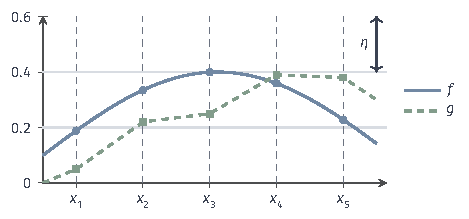
\includegraphics[width=79.4mm]{figures/02-abstract-mathematics/03-function-spaces/tikz/c6-lipschitz-quantization/figure.pdf}
  \caption{Lipschitz类的网格量化，$L=1$，$\varepsilon=0.4$。竖虚线为网格点$x_1,\ldots,x_5$，相邻间距$2\delta=0.2$，每点到最近网格点不超过$\delta=\varepsilon/(4L)$；横线把值域分为高$\eta=\varepsilon/2$的层（图中只画出非负部分）。$f(x)=0.1+0.3\sin3x$（蓝）与折线$g$（绿）在每个网格点处落在同一层，即记录相同，二者一致距离不超过$2L\delta+\eta=\varepsilon$。}
  \label{fig:apx-lipschitz-quantization}
\end{figure}

定义域的覆盖数出现在指数上。对$X=[0,1]$，$p=\lceil1/(2\delta)\rceil=\lceil2L/\varepsilon\rceil$，得到
\[
  \log N(\varepsilon,\mathcal F_{L,M},d_\infty)\le\Bigl\lceil\frac{2L}\varepsilon\Bigr\rceil\log\Bigl\lceil\frac{4M}\varepsilon\Bigr\rceil .
\]
与有限维参数族的$p\log(1/\varepsilon)$相比，这里的“有效维数”$\lceil2L/\varepsilon\rceil$随精度增长，Lipschitz类是无限维的。对$X=[0,1]^d$，网格点个数按$(L/\varepsilon)^d$增长，度量熵也随之增长，这是与张量积网格同源的维数效应。这个上界并不最优：Kolmogorov与Tikhomirov证明，固定$L$、$M$时，$[0,1]^d$上有界Lipschitz类的度量熵在$\varepsilon\to0$时与$\varepsilon^{-d}$同阶，上界中多出的对数因子可以去掉\scite{kolmogorov1959epsilon}。这里的构造只用来说明有限覆盖如何从共同的正则性和幅度约束中产生。

\paragraph{覆盖数之外的容量与保证}

覆盖数总是相对于一个预先固定的距离和精度定义的。学习理论中还会遇到其他容量量：伪维和胖打散维数检查一个类在有限输入上能实现多少种跨越阈值的模式，序贯覆盖数在依赖历史的查询树上计数。它们的评价对象与覆盖数不同，不能从名称相近而互换。覆盖数本身也不提供统计误差或预测保证；要得到这类结论，还需加入随机样本、损失函数和集中不等式，可参考\BookChapterRef{chap:statistical-learning-framework}{卷六“机器学习理论基础”章}。
